\chapter{Classification}

\begin{Definition}[Classification]
Raisonnement \textbf{à partir de cas} : on a des enregistrements décrits par des attributs,
dont l'un est la \textbf{classe}. On cherche un \textbf{modèle} qui exprime la classe en
fonction des autres attributs, pour ensuite \textbf{prédire la classe} d'enregistrements
inconnus. C'est de l'apprentissage \textbf{supervisé}.
\end{Definition}

\textbf{Deux étapes :} (1) \emph{construction du modèle} sur l'ensemble d'\textbf{apprentissage}
(\emph{training set}, $\approx 2/3$) ; (2) \emph{utilisation/test} du modèle sur l'ensemble de
\textbf{test} ($\approx 1/3$) pour mesurer la précision. On peut aussi faire de la
\textbf{validation croisée} : découper en $k$ paquets, apprendre sur $k-1$ et tester sur le
dernier, en tournant.

\section{Méthode des $K$ plus proches voisins (K-NN)}

\begin{Definition}[K-NN]
\textbf{Pas d'apprentissage} : le modèle \emph{est} l'échantillon. Pour classer un nouvel
individu $y$ : on calcule sa \textbf{distance} à tous les individus connus, on garde les
\textbf{$K$ plus proches}, et on attribue à $y$ la \textbf{classe majoritaire} parmi ces $K$
voisins. Heuristique : $K = \text{nombre d'attributs} + 1$.
\end{Definition}

\textbf{Vote simple} : chaque voisin compte pour 1. \textbf{Vote pondéré} : chaque voisin a un
poids $\propto 1/\text{distance}$ (plus il est proche, plus il pèse). \textbf{Confiance} $=$
votes gagnants $/$ total des votes.

\textbf{Distances entre numériques} ($x,y\in\R^m$) :
\[ d_{\text{Euclidienne}}=\sqrt{\textstyle\sum_i (x_i-y_i)^2},\quad
   d_{\text{Manhattan}}=\textstyle\sum_i |x_i-y_i|,\quad
   d_{\text{Minkowski}}=\Big(\textstyle\sum_i |x_i-y_i|^q\Big)^{1/q}. \]
($q=1$ : Manhattan ; $q=2$ : Euclidienne.) \textbf{Données nominales} : $d=0$ si égales, $1$
sinon.

\begin{Attention}
K-NN dépend des distances : il faut \textbf{normaliser} les attributs avant, sinon
l'attribut aux grandes valeurs (ex. le salaire) écrase les autres.
\end{Attention}

\subsection{Exercice résolu — classer David ($K=3$, euclidienne)}
\begin{center}\small
\begin{tabular}{lcccc}
\toprule
Client & Âge & Salaire & Nb cartes & Classe (Loyal)\\
\midrule
Jean & 35 & 35000 & 3 & N\\
Rachèle & 22 & 50000 & 2 & O\\
Anne & 63 & 200000 & 1 & N\\
Thomas & 59 & 170000 & 1 & N\\
Nathalie & 25 & 40000 & 4 & O\\
\rowcolor{orangeclair}\textbf{David} & 37 & 50000 & 2 & \textbf{?}\\
\bottomrule
\end{tabular}
\end{center}

\textbf{Démarche, en 3 temps :} (1) on calcule la distance de David à \emph{chacun} des 5
clients connus ; (2) on \emph{trie} ces distances et on garde les $K=3$ plus petites ;
(3) on regarde la classe de ces 3 voisins et on \emph{vote}.

\begin{Calcul}[: distances euclidiennes de David $(37;50000;2)$ à chacun]
On applique $d=\sqrt{(\Delta\text{âge})^2+(\Delta\text{salaire})^2+(\Delta\text{cartes})^2}$.
On écrit \emph{tous} les termes avant de simplifier :
\begin{align*}
d(\text{David},\text{Jean}) &=\sqrt{(37-35)^2+(50000-35000)^2+(2-3)^2}
   =\sqrt{\underbrace{4}_{\text{âge}}+\underbrace{225\,000\,000}_{\text{salaire}}+\underbrace{1}_{\text{cartes}}}\approx \mathbf{15000{,}0}\\
d(\text{David},\text{Rachèle}) &=\sqrt{(37-22)^2+(50000-50000)^2+(2-2)^2}
   =\sqrt{225+0+0}= \mathbf{15{,}0}\\
d(\text{David},\text{Anne}) &=\sqrt{(37-63)^2+(50000-200000)^2+(2-1)^2}
   =\sqrt{676+22\,500\,000\,000+1}\approx \mathbf{150000{,}0}\\
d(\text{David},\text{Thomas}) &=\sqrt{(37-59)^2+(50000-170000)^2+(2-1)^2}
   =\sqrt{484+14\,400\,000\,000+1}\approx \mathbf{120000{,}0}\\
d(\text{David},\text{Nathalie}) &=\sqrt{(37-25)^2+(50000-40000)^2+(2-4)^2}
   =\sqrt{144+100\,000\,000+4}\approx \mathbf{10000{,}0}
\end{align*}
\textbf{Tri croissant} : Rachèle $15$ < Nathalie $10\,000$ < Jean $15\,000$ < Thomas
$120\,000$ < Anne $150\,000$. \\
\textbf{Les $K=3$ plus proches} : Rachèle (\textbf{O}), Nathalie (\textbf{O}), Jean (\textbf{N}).
\end{Calcul}

\begin{Calcul}[: vote simple — détail]
On compte les classes des 3 voisins : \og O \fg{} apparaît 2 fois (Rachèle, Nathalie),
\og N \fg{} 1 fois (Jean).
\[ \text{score}(O)=2,\qquad \text{score}(N)=1 \;\Rightarrow\; \text{classe majoritaire}=\mathbf{O}. \]
\textbf{Confiance} $=\dfrac{\text{voix gagnantes}}{\text{total des voix}}=\dfrac{2}{3}\approx \mathbf{67\,\%}$.
\end{Calcul}

\begin{Calcul}[: vote pondéré — détail]
Chaque voisin pèse $w=1/d$ (proche $\Rightarrow$ gros poids). On additionne les poids
\emph{par classe} :
\[ w_O=\underbrace{\tfrac{1}{15}}_{\text{Rachèle}}+\underbrace{\tfrac{1}{10000}}_{\text{Nathalie}}
   \approx 0{,}06667+0{,}00010=0{,}06677, \qquad
   w_N=\underbrace{\tfrac{1}{15000}}_{\text{Jean}}\approx 0{,}00007. \]
Comme $w_O \gg w_N$, la classe pondérée est \textbf{O}.
Confiance pondérée $=\dfrac{w_O}{w_O+w_N}=\dfrac{0{,}06677}{0{,}06684}\approx \mathbf{99{,}9\,\%}$.
\textbf{Conclusion identique :} David est classé \textbf{O} (Loyal $=$ O).
\end{Calcul}

\begin{Attention}[: le piège des échelles]
Regardez les termes sous la racine : le salaire pèse $\sim 10^8$, l'âge $\sim 10^2$, les
cartes $\sim 1$. \textbf{Le salaire écrase tout} : la distance est, à $0{,}001\,\%$ près, égale
à l'écart de salaire. On ne fait donc, en réalité, du K-NN \emph{que sur le salaire}. C'est
pourquoi le cours recommande de \textbf{normaliser avant un K-NN}.
\end{Attention}

\begin{Calcul}[: la même classification, mais \textbf{normalisée} (min-max)]
On ramène chaque attribut dans $[0,1]$ avec $x^*=\dfrac{x-\min}{\max-\min}$, à partir des
bornes de l'apprentissage : âge $\in[22,63]$ (étendue 41), salaire $\in[35000,200000]$
(étendue 165000), cartes $\in[1,4]$ (étendue 3).\\[3pt]
David $\rightarrow \big(\tfrac{37-22}{41};\tfrac{50000-35000}{165000};\tfrac{2-1}{3}\big)
=(0{,}366;\,0{,}091;\,0{,}333)$. Distances normalisées :
\begin{center}\small
\begin{tabular}{lccccc}
\toprule
& Jean & Rachèle & Anne & Thomas & Nathalie\\
\midrule
distance & \textbf{0,349} (N) & \textbf{0,366} (O) & 1,157 (N) & 0,963 (N) & \textbf{0,731} (O)\\
\bottomrule
\end{tabular}
\end{center}
\textbf{Surprise :} maintenant que les 3 attributs comptent autant, \textbf{Jean (N) devient le
plus proche} ! Mais les 3 plus proches sont Jean (N), Rachèle (O), Nathalie (O) : le vote
donne encore $\mathbf{O}$ (2 contre 1). La normalisation a changé les distances et le
classement, \textbf{pas la décision finale} ici.
\end{Calcul}

\begin{figure}[ht]\centering
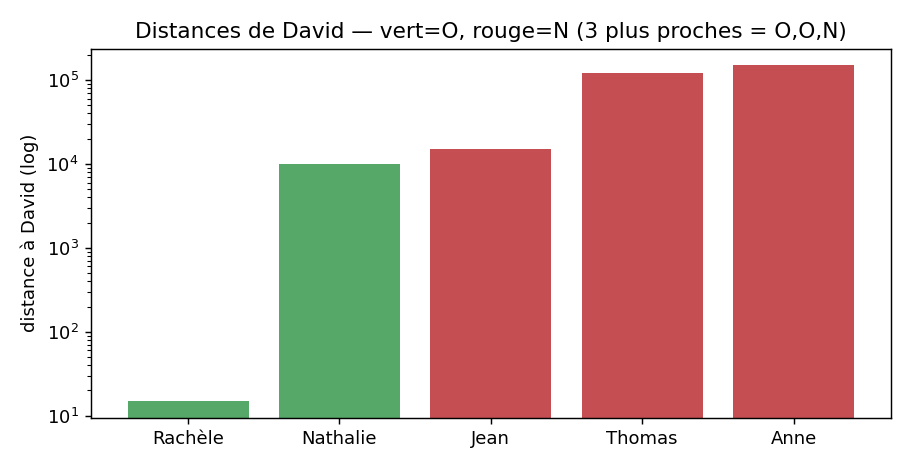
\includegraphics[width=0.7\linewidth]{figures/knn_distances.png}
\caption{Distances brutes de David (échelle log à cause du salaire). Vert $=$ O, rouge $=$ N.
Les 3 plus proches : O, O, N $\Rightarrow$ O.}
\end{figure}

\lstinputlisting[caption={scripts/knn\_david.py},label=lst:knn]{../scripts/knn_david.py}

\section{Arbres de décision}

\begin{Definition}[Arbre de décision]
Représentation graphique d'une procédure de classification. \textbf{Nœud interne} $=$ test
sur un attribut ; \textbf{branche} $=$ résultat du test ; \textbf{feuille} $=$ classe. Chaque
chemin racine$\rightarrow$feuille donne une \textbf{règle SI…ALORS}.
\end{Definition}

\textbf{Construction (récursive)} : (1) toutes les instances à la racine ; (2) choisir le
\textbf{meilleur attribut} de découpage (selon un critère) ; (3) partitionner ; (4) recommencer
sur chaque fils ; (5) arrêter quand le nœud est \textbf{pur} (une seule classe), presque pur,
ou qu'il n'y a plus d'attribut. Critères de choix : \textbf{indice de Gini} (CART),
\textbf{gain d'information} (ID3, C4.5), $\chi^2$ (CHAID).

\subsection{Critère 1 — Indice de Gini}

\begin{Definition}[Gini]
\[ GINI(t)=1-\sum_j \big[p(j|t)\big]^2 \]
$p(j|t)$ $=$ fréquence de la classe $j$ au nœud $t$. \textbf{Gini $=0$} si le nœud est
\textbf{pur} ; plus Gini est \textbf{bas}, plus le nœud est \textbf{pur}.
Pour un découpage en $k$ fils :
\[ GINI_{\text{split}}=\sum_{i=1}^{k}\frac{n_i}{n}\,GINI(i) \quad\text{(à \textbf{minimiser})}. \]
\end{Definition}

\begin{Calcul}[: petits exemples de Gini (sur 6 enregistrements)]
$(C_1{=}0,C_2{=}6)$ : $GINI=1-0^2-1^2=\mathbf{0}$ (pur).\quad
$(C_1{=}1,C_2{=}5)$ : $GINI=1-(\tfrac16)^2-(\tfrac56)^2=\mathbf{0{,}278}$.\quad
$(C_1{=}2,C_2{=}4)$ : $GINI=1-(\tfrac26)^2-(\tfrac46)^2=\mathbf{0{,}444}$.
\end{Calcul}

\paragraph{Exercice résolu (assurance auto).}
\begin{center}\small
\begin{tabular}{ccc}
\toprule
Âge & Type\_voit & Risque\\
\midrule
23 & Familiale & Élevé\\ 17 & Sport & Élevé\\ 43 & Sport & Élevé\\
68 & Familiale & Faible\\ 32 & Camion & Faible\\ 20 & Familiale & Élevé\\
\bottomrule
\end{tabular}
\end{center}

\textbf{Plan :} on évalue chaque attribut comme candidat de découpage de la racine, on garde
celui qui donne le plus petit $GINI_{\text{split}}$, puis on recommence sur chaque fils.

\begin{Calcul}[: étape 0 — impureté de la racine]
La racine contient les 6 enregistrements : 4 \og Élevé \fg{} et 2 \og Faible \fg{}. Les
fréquences sont $p(\text{Élevé})=\tfrac46$ et $p(\text{Faible})=\tfrac26$, donc
\[ GINI(\text{racine})=1-\Big(\tfrac46\Big)^2-\Big(\tfrac26\Big)^2
   =1-\tfrac{16}{36}-\tfrac{4}{36}=1-0{,}444-0{,}111=\mathbf{0{,}444}. \]
\textbf{But :} trouver le découpage qui fait \emph{le plus baisser} cette valeur.
\end{Calcul}

\begin{Calcul}[: candidat A — l'attribut nominal \texttt{Type\_voit}]
Découpage multi-branche, un fils par valeur :
\begin{itemize}[nosep,leftmargin=1.4em]
  \item \textbf{Familiale} $=\{$Élevé (23), Faible (68), Élevé (20)$\}$ : 2 Élevé, 1 Faible,
        donc $GINI=1-(\tfrac23)^2-(\tfrac13)^2=1-0{,}444-0{,}111=0{,}444$ ;
  \item \textbf{Sport} $=\{$Élevé (17), Élevé (43)$\}$ : \emph{pur} $\Rightarrow GINI=0$ ;
  \item \textbf{Camion} $=\{$Faible (32)$\}$ : \emph{pur} $\Rightarrow GINI=0$.
\end{itemize}
Moyenne pondérée par la taille des fils ($3,2,1$ sur $6$) :
\[ GINI_{\text{split}}=\tfrac36(0{,}444)+\tfrac26(0)+\tfrac16(0)=\mathbf{0{,}222}. \]
\end{Calcul}

\begin{Calcul}[: candidat B — l'attribut continu \texttt{Âge} (on teste \emph{tous} les seuils)]
On trie les âges et leur classe : $17_{\text{É}}, 20_{\text{É}}, 23_{\text{É}}, 32_{\text{F}},
43_{\text{É}}, 68_{\text{F}}$. Un seuil candidat est le \emph{milieu} de deux âges consécutifs.
\begin{center}\small
\renewcommand{\arraystretch}{1.3}
\begin{tabular}{c l l c}
\toprule
Seuil & Gauche (Âge $<$ seuil) & Droite (Âge $\geq$ seuil) & $GINI_{\text{split}}$\\
\midrule
18,5 & $\{17\}$ : É — pur, $0$ & $\{20,23,32,43,68\}$ : 3É,2F, $0{,}48$ &
  $\tfrac16(0)+\tfrac56(0{,}48)=0{,}400$\\
21,5 & $\{17,20\}$ : pur, $0$ & $\{23,32,43,68\}$ : 2É,2F, $0{,}50$ &
  $\tfrac26(0)+\tfrac46(0{,}50)=0{,}333$\\
\rowcolor{vertclair}\textbf{27,5} & $\{17,20,23\}$ : pur, $0$ & $\{32,43,68\}$ : 1É,2F, $0{,}444$ &
  $\tfrac36(0)+\tfrac36(0{,}444)=\mathbf{0{,}222}$\\
37,5 & $\{17,20,23,32\}$ : 3É,1F, $0{,}375$ & $\{43,68\}$ : 1É,1F, $0{,}50$ &
  $\tfrac46(0{,}375)+\tfrac26(0{,}50)=0{,}417$\\
55,5 & $\{17,20,23,32,43\}$ : 4É,1F, $0{,}32$ & $\{68\}$ : pur, $0$ &
  $\tfrac56(0{,}32)+\tfrac16(0)=0{,}267$\\
\bottomrule
\end{tabular}
\end{center}
Le \textbf{meilleur seuil} est $\text{Âge}<27{,}5$ avec $GINI_{\text{split}}=\mathbf{0{,}222}$
(détail d'un $GINI$ de fils : pour la droite $\{32,43,68\}$, 1 Élevé et 2 Faible donnent
$1-(\tfrac13)^2-(\tfrac23)^2=0{,}444$).
\end{Calcul}

\begin{Astuce}[: pourquoi Âge $<27{,}5$ et pas \texttt{Type\_voit} ?]
Les deux donnent $GINI_{\text{split}}=0{,}222$ : \textbf{égalité parfaite}. En cas d'égalité,
CART/scikit-learn tranche selon l'ordre interne des variables et choisit ici
\textbf{Âge $<27{,}5$}. On suit ce choix (l'autre arbre, démarrant par \texttt{Type\_voit},
serait tout aussi correct).
\end{Astuce}

\begin{Calcul}[: 2\textsuperscript{e} niveau — le fils \og Âge $\geq 27{,}5$ \fg{}]
Le fils gauche (\og Âge $<27{,}5$ \fg{}) est \emph{pur} (tous Élevé) : c'est une feuille,
on s'arrête. Le fils droit contient $\{32_{\text{Camion,F}}, 43_{\text{Sport,É}},
68_{\text{Familiale,F}}\}$, soit 1 Élevé et 2 Faible : $GINI=0{,}444$, il faut le re-découper.
\begin{itemize}[nosep,leftmargin=1.4em]
  \item \textbf{Par \texttt{Type\_voit}} : Sport$\to\{$É$\}$ pur, Familiale$\to\{$F$\}$ pur,
        Camion$\to\{$F$\}$ pur. $GINI_{\text{split}}=\mathbf{0}$ — \textbf{séparation parfaite}.
  \item \textbf{Par \texttt{Âge}} (seuils 37,5 et 55,5) : on retombe à chaque fois sur
        $GINI_{\text{split}}=\tfrac13(0)+\tfrac23(0{,}5)=0{,}333$.
\end{itemize}
$0 < 0{,}333$ : on choisit donc \texttt{Type\_voit}, qui classe parfaitement les 3 derniers cas.
\end{Calcul}

\begin{Exemple}[arbre Gini final]
{\ttfamily\setlength{\parindent}{0pt}
Âge < 27,5 ?\\
\quad |-- OUI ~~> \textbf{Élevé}\\
\quad |-- NON ~~> Type\_voit ?\\
\quad\qquad\quad |-- Sport ~~> \textbf{Élevé}\\
\quad\qquad\quad |-- Familiale ~~> \textbf{Faible}\\
\quad\qquad\quad |-- Camion ~~> \textbf{Faible}
}
\end{Exemple}

\begin{figure}[ht]\centering
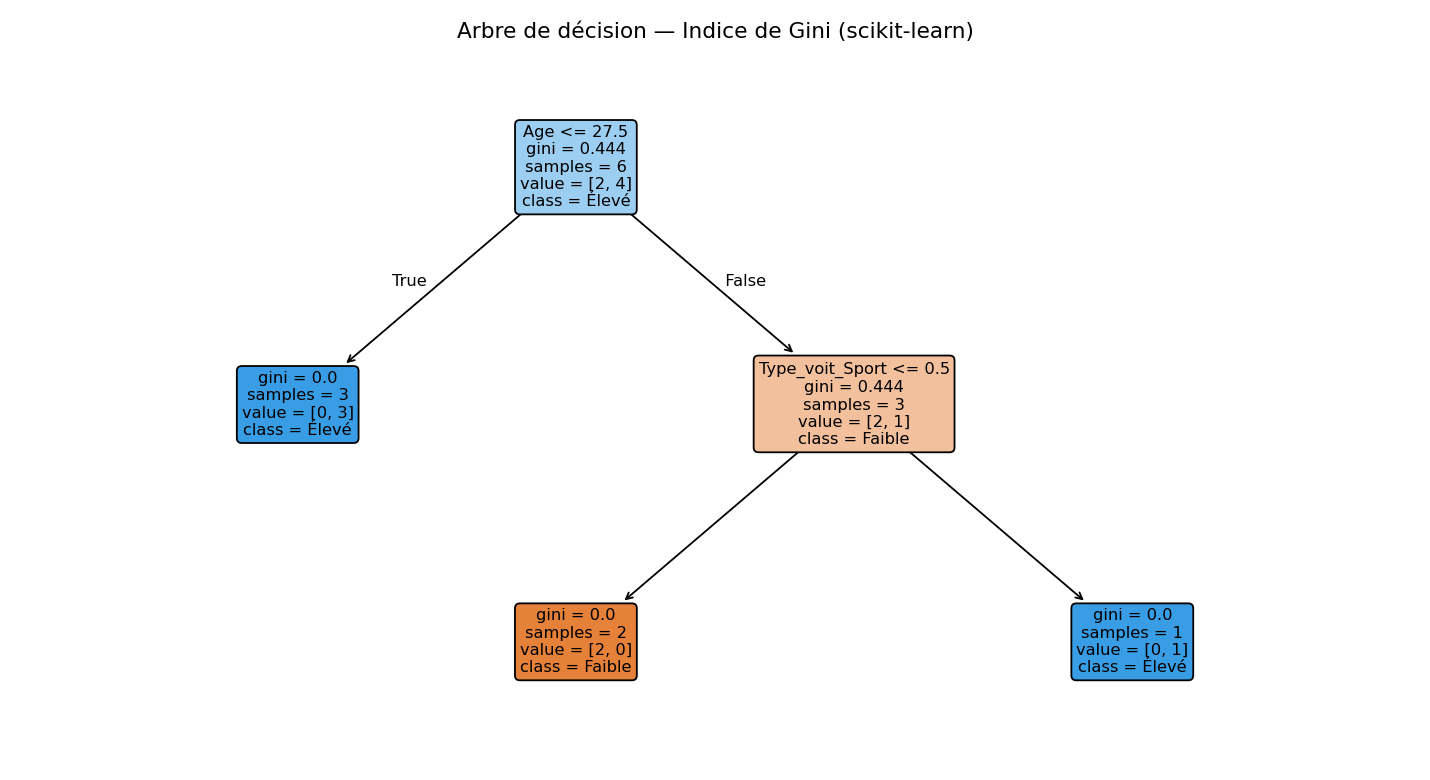
\includegraphics[width=0.85\linewidth]{figures/gini_arbre.png}
\caption{Arbre de décision Gini reconstruit par scikit-learn (\texttt{Type\_voit} encodé en one-hot).}
\end{figure}

\lstinputlisting[caption={scripts/gini\_arbre.py},label=lst:gini]{../scripts/gini_arbre.py}

\subsection{Critère 2 — Gain d'information (entropie)}

\begin{Definition}[Entropie et gain]
\[ Entropie(t)=-\sum_j p(j|t)\log_2 p(j|t),\qquad
   GAIN_{\text{split}}=Entropie(p)-\sum_{i=1}^{k}\frac{n_i}{n}Entropie(i). \]
Entropie $=0$ si pur, maximale ($\log_2 n_c$) si classes équilibrées. On choisit l'attribut
qui \textbf{maximise le gain} (la plus grande réduction d'entropie). \textbf{C4.5} corrige en
divisant par le \emph{SplitINFO} (\emph{gain ratio}) pour pénaliser les attributs à trop de
valeurs.
\end{Definition}

\begin{Calcul}[: comprendre l'entropie sur 3 cas (6 enregistrements)]
On note $\log_2 x=\dfrac{\ln x}{\ln 2}$. Plus le mélange est équilibré, plus l'entropie est grande.
\begin{itemize}[nosep,leftmargin=1.4em]
  \item $(C_1{=}0,C_2{=}6)$ : tout dans une classe.
        $-\tfrac06\log_2\tfrac06-\tfrac66\log_2\tfrac66=-0-1\cdot\log_2 1=-0-0=\mathbf{0}$
        (nœud \emph{pur}).
  \item $(C_1{=}1,C_2{=}5)$ : $-\tfrac16\log_2\tfrac16-\tfrac56\log_2\tfrac56
        =-\tfrac16(-2{,}585)-\tfrac56(-0{,}263)=0{,}431+0{,}219=\mathbf{0{,}650}$.
  \item $(C_1{=}2,C_2{=}4)$ : $-\tfrac26\log_2\tfrac26-\tfrac46\log_2\tfrac46
        =-\tfrac13(-1{,}585)-\tfrac23(-0{,}585)=0{,}528+0{,}390=\mathbf{0{,}918}$.
\end{itemize}
\end{Calcul}

\paragraph{Exercice résolu (achat d'ordinateur, 14 individus).} C'est l'exemple du TP.
Classe \texttt{Achète\_ordinateur} : \textbf{9 \og oui \fg{}} et \textbf{5 \og non \fg{}}.

\begin{Calcul}[: étape 0 — entropie de la racine]
\[ Entropie(S)=-\tfrac{9}{14}\log_2\tfrac{9}{14}-\tfrac{5}{14}\log_2\tfrac{5}{14}
   =-0{,}643\cdot(-0{,}637)-0{,}357\cdot(-1{,}485)=0{,}410+0{,}530=\mathbf{0{,}940}. \]
\end{Calcul}

\begin{Calcul}[: gain de l'attribut \texttt{Âge}]
\texttt{Âge} a 3 valeurs. On compte les classes dans chaque groupe, puis son entropie :
\begin{itemize}[nosep,leftmargin=1.4em]
  \item $\le 30$ : 5 individus, \textbf{2 oui / 3 non} $\Rightarrow
        -\tfrac25\log_2\tfrac25-\tfrac35\log_2\tfrac35=0{,}529+0{,}442=0{,}971$ ;
  \item $31..40$ : 4 individus, \textbf{4 oui / 0 non} $\Rightarrow$ pur, entropie $=0$ ;
  \item $>40$ : 5 individus, \textbf{3 oui / 2 non} $\Rightarrow 0{,}971$ (symétrique du premier).
\end{itemize}
Entropie restante (pondérée par $5,4,5$ sur $14$) :
\[ E_{\text{reste}}=\tfrac{5}{14}(0{,}971)+\tfrac{4}{14}(0)+\tfrac{5}{14}(0{,}971)=0{,}694
   \;\Rightarrow\; \boxed{GAIN(\text{Âge})=0{,}940-0{,}694=0{,}247}. \]
\end{Calcul}

\begin{Calcul}[: gain des trois autres attributs]
\textbf{\texttt{Revenue}} (élevé : 2o/2n $\to1{,}0$ ; moyen : 4o/2n $\to0{,}918$ ; bas : 3o/1n $\to0{,}811$) :
\[ E_{\text{reste}}=\tfrac{4}{14}(1)+\tfrac{6}{14}(0{,}918)+\tfrac{4}{14}(0{,}811)=0{,}911
   \;\Rightarrow\; GAIN=\mathbf{0{,}029}. \]
\textbf{\texttt{Étudiant}} (oui : 6o/1n $\to0{,}592$ ; non : 3o/4n $\to0{,}985$) :
\[ E_{\text{reste}}=\tfrac{7}{14}(0{,}592)+\tfrac{7}{14}(0{,}985)=0{,}789
   \;\Rightarrow\; GAIN=\mathbf{0{,}151}. \]
\textbf{\texttt{État\_civil}} (célibataire : 6o/2n $\to0{,}811$ ; marié : 3o/3n $\to1{,}0$) :
\[ E_{\text{reste}}=\tfrac{8}{14}(0{,}811)+\tfrac{6}{14}(1)=0{,}892
   \;\Rightarrow\; GAIN=\mathbf{0{,}048}. \]
\end{Calcul}

\begin{Astuce}[: choix de la racine]
\begin{center}\small
\begin{tabular}{lcccc}
\toprule
Attribut & \textbf{Âge} & Étudiant & État\_civil & Revenue\\
\midrule
Gain & \cellcolor{vertclair}\textbf{0,247} & 0,151 & 0,048 & 0,029\\
\bottomrule
\end{tabular}
\end{center}
\texttt{Âge} a le \textbf{plus grand gain} (réduit le plus l'entropie) : c'est la \textbf{racine}.
\end{Astuce}

\begin{Calcul}[: 2\textsuperscript{e} niveau — re-découper chaque fils de l'âge]
\textbf{Âge $=31..40$} : déjà pur (4 oui) $\Rightarrow$ \textbf{feuille \og oui \fg{}}, on s'arrête.\\[3pt]
\textbf{Âge $\le 30$} (2 oui, 3 non, entropie $0{,}971$). On recalcule le gain des attributs
\emph{restants} dans ce sous-ensemble de 5 individus :
\begin{itemize}[nosep,leftmargin=1.4em]
  \item \texttt{Étudiant} : oui$\to\{$oui,oui$\}$ (pur), non$\to\{$non,non,non$\}$ (pur)
        $\Rightarrow E_{\text{reste}}=0$, \textbf{gain $=0{,}971$ (maximal)} ;
  \item \texttt{Revenue} : gain $=0{,}571$ ; \quad \texttt{État\_civil} : gain $=0{,}020$.
\end{itemize}
$\Rightarrow$ on découpe sur \textbf{\texttt{Étudiant}} (sépare parfaitement).\\[3pt]
\textbf{Âge $>40$} (3 oui, 2 non, entropie $0{,}971$) :
\begin{itemize}[nosep,leftmargin=1.4em]
  \item \texttt{État\_civil} : célibataire$\to\{$3 oui$\}$ (pur), marié$\to\{$2 non$\}$ (pur)
        $\Rightarrow$ \textbf{gain $=0{,}971$ (maximal)} ;
  \item \texttt{Étudiant} : gain $=0{,}020$ ; \quad \texttt{Revenue} : gain $=0{,}020$.
\end{itemize}
$\Rightarrow$ on découpe sur \textbf{\texttt{État\_civil}} (sépare parfaitement).
\end{Calcul}

\begin{Exemple}[arbre gain d'information final]
{\ttfamily\setlength{\parindent}{0pt}
Âge ?\\
\quad |-- (<= 30) ~~> Étudiant ?~~ oui ~~> \textbf{oui} ~/~ non ~~> \textbf{non}\\
\quad |-- (31..40) ~~> \textbf{oui}\\
\quad |-- (> 40) ~~> État\_civil ?~~ célibataire ~~> \textbf{oui} ~/~ marié ~~> \textbf{non}
}
\end{Exemple}

\begin{figure}[ht]\centering
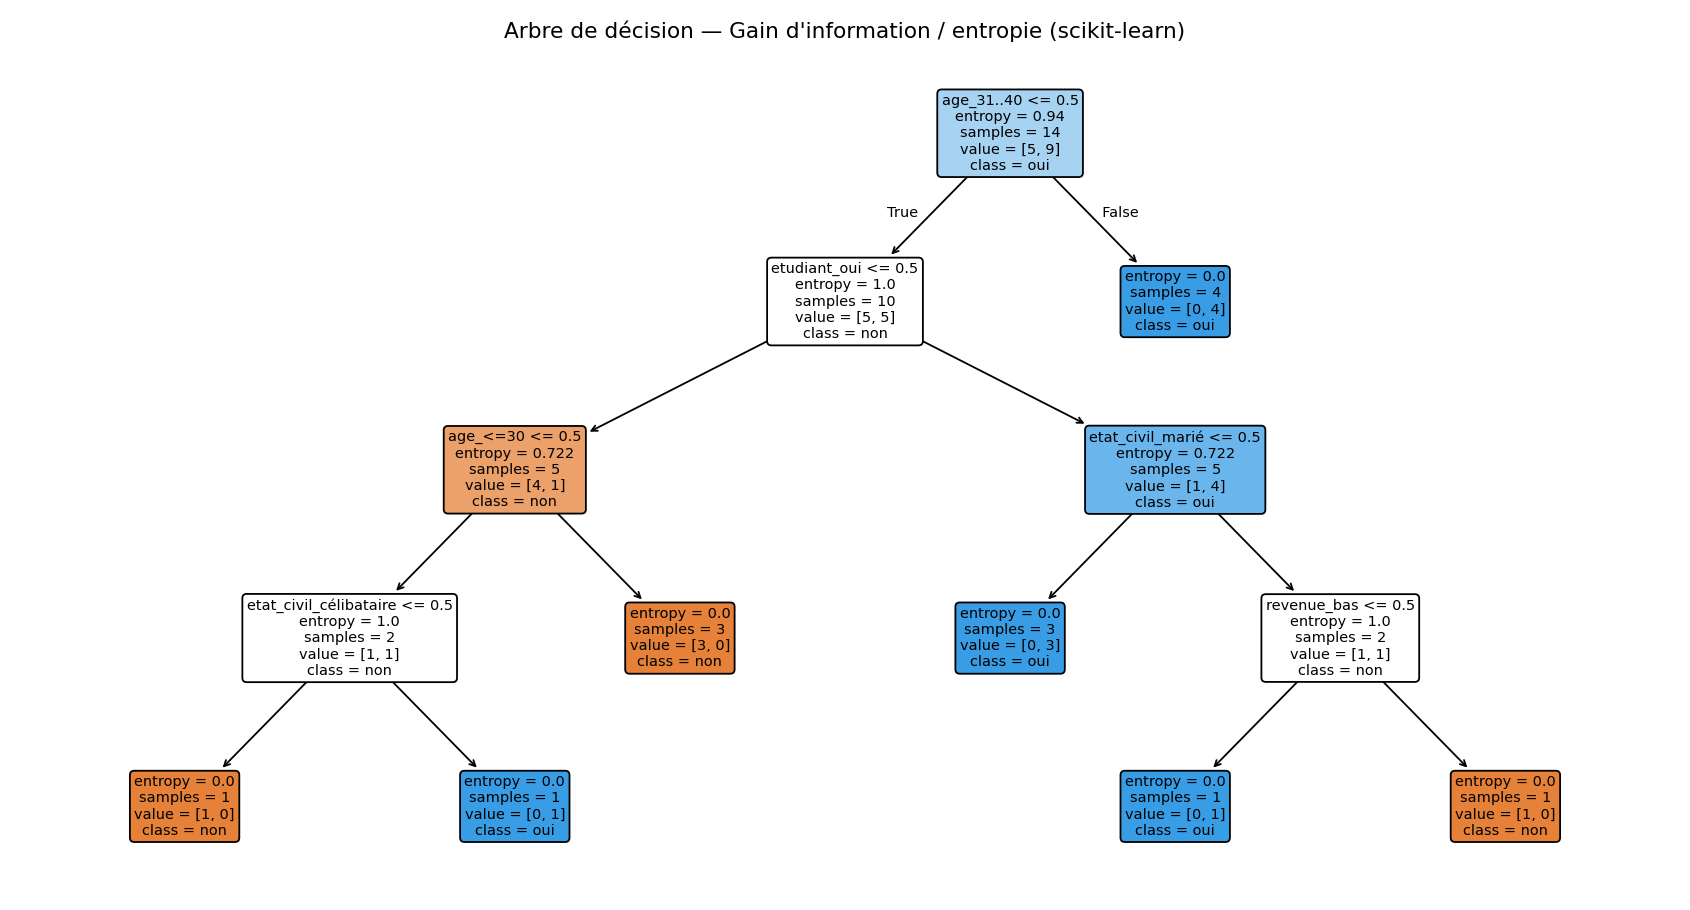
\includegraphics[width=\linewidth]{figures/gain_information_arbre.png}
\caption{Arbre par gain d'information (entropie) reconstruit par scikit-learn.}
\end{figure}

\lstinputlisting[caption={scripts/gain\_information.py},label=lst:gain]{../scripts/gain_information.py}

\section{Mesures de performance}

À partir de la \textbf{matrice de confusion} (cas binaire) :
\begin{center}
\begin{tabular}{l|cc}
& prédit positif & prédit négatif\\\hline
réel positif & TP (vrais positifs) & FN (faux négatifs)\\
réel négatif & FP (faux positifs) & TN (vrais négatifs)\\
\end{tabular}
\end{center}

\[ \text{Exactitude}=\frac{TP+TN}{TP+TN+FP+FN},\quad
   \text{Précision}=\frac{TP}{TP+FP},\quad
   \text{Rappel}=\frac{TP}{TP+FN} \]
\[ \text{Spécificité}=\frac{TN}{TN+FP},\qquad
   F_1=\frac{2\cdot \text{Précision}\cdot \text{Rappel}}{\text{Précision}+\text{Rappel}}. \]

\begin{Calcul}[: exemple TP=40, FN=10, FP=5, TN=45]
Exactitude $=\tfrac{40+45}{100}=0{,}85$ ; Précision $=\tfrac{40}{45}=0{,}889$ ;
Rappel $=\tfrac{40}{50}=0{,}80$ ; Spécificité $=\tfrac{45}{50}=0{,}90$ ;
$F_1=\tfrac{2\cdot0{,}889\cdot0{,}80}{0{,}889+0{,}80}=0{,}842$.
\end{Calcul}

\textbf{Multi-classes} : matrice $m\times m$, bonnes affectations $S=\sum_i n_{ii}$ (diagonale),
taux d'erreur $E=1-\frac{\sum_i n_{ii}}{\sum_{i,j} n_{ij}}$.

\begin{figure}[ht]\centering
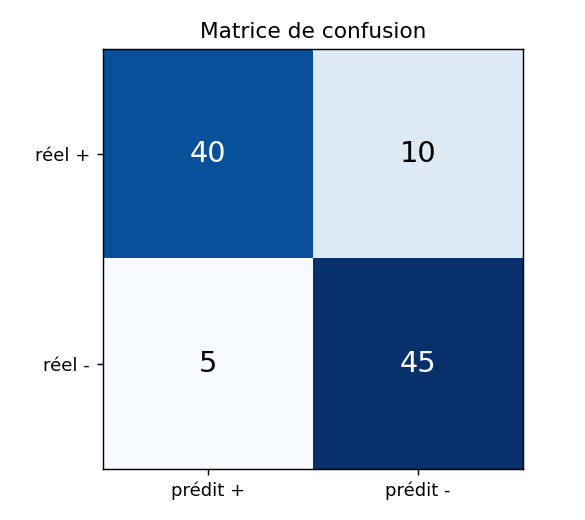
\includegraphics[width=0.4\linewidth]{figures/matrice_confusion.png}
\caption{Matrice de confusion de l'exemple.}
\end{figure}

\lstinputlisting[caption={scripts/performance\_classification.py},label=lst:perf]{../scripts/performance_classification.py}

\begin{Resume}
\textbf{K-NN} : pas d'apprentissage, on vote parmi les $K$ voisins les plus proches
(normaliser avant !). \textbf{Arbres} : on découpe récursivement selon le meilleur attribut —
\textbf{Gini} (à minimiser, CART) ou \textbf{gain d'information} (à maximiser, ID3/C4.5).
\textbf{Performance} : matrice de confusion $\rightarrow$ exactitude, précision, rappel, $F_1$.
\end{Resume}
